\documentclass{article}
\usepackage[margin=1in]{geometry}
\usepackage{amsmath,amsthm,amssymb}
\usepackage{bbm,enumerate,mathtools}
\usepackage{tikz,pgfplots}
\usepackage{chessboard}
\usepackage[hidelinks]{hyperref}
\usepackage{multicol} % Problem 35

\newenvironment{question}{\begin{trivlist}\item[\textbf{Question.}]}{\end{trivlist}}
\newenvironment{note}{\begin{trivlist}\item[\textbf{Note.}]}{\end{trivlist}}
\newenvironment{references}{\begin{trivlist}\item[\textbf{References.}]}{\end{trivlist}}
\newenvironment{related}{\begin{trivlist}\item[\textbf{Related.}]\end{trivlist}\begin{enumerate}}{\end{enumerate}}


\begin{document}
\rating{3}{3}
Consider a puzzle on a (blank) $n \times m$ board, where each column and row
has a number denoting the number of markers that should go in that column or
row. The player's goal is to fill in the grid in such a way that the
row/column ``histograms'' are satisfied.
\begin{figure}[!h]
  \centering
  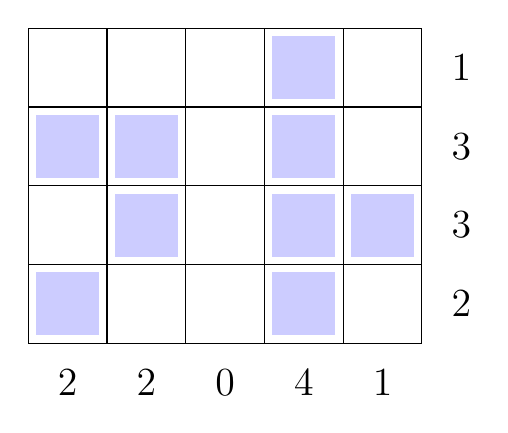
\begin{tikzpicture}
    \draw (0,0) grid (5,4);
    \foreach \x/\label in {0/2, 1/2, 2/0, 3/4, 4/1} {
      \node at ({\x + 0.5}, -0.5) {\Large \label};
    }
    \foreach \y/\label in {0/2, 1/3, 2/3, 3/1} {
      \node at (5.5, {\y + 0.5}) {\Large \label};
    }
    \foreach \x/\y in {0/0, 0/2, 1/1, 1/2, 3/0, 3/1, 3/2, 3/3, 4/1} {
      \fill[blue!20] ({\x + 0.1}, {\y + 0.1}) rectangle ({\x + 0.9}, {\y + 0.9});
    }
  \end{tikzpicture}
  \caption{
    Example of a solution to the puzzle $(2, 2, 0, 4, 1) \times (1, 3, 3, 2)$.
    Is the solution unique?
  }
\end{figure}
\begin{question}
  What is a procedure for determining if a grid has a solution? If it has a
  unique solution?
\end{question}
\begin{related}
  \item What if the game is played on a $d$-dimensional hypercube?
  \item What if the game is played on a triangle? Tetrahedron?
  \item What is the greatest amount of ambiguity a non-unique board can have?
    (i.e. what is the greatest number of solutions?)
  \item How many maximally ambiguous boards exist?
  \item How many distinct boards exist up to dihedral action?
    Up to torus action?
  \item What if multiple markers can be put in each cell?
\end{related}
\begin{references}
  \item \url{https://oeis.org/A297077}
\end{references}

\end{document}
